\documentclass[a4paper,11pt]{scrartcl}

\usepackage[ngerman]{babel}
\PassOptionsToPackage{hyphens}{url}\usepackage[hidelinks]{hyperref}
\usepackage{graphicx}
\usepackage{longtable}
\usepackage{tabularx}
%\usepackage[top=1.5cm,right=1.5cm,bottom=2.5cm,left=1.5cm]{geometry}
\usepackage{gensymb}
\usepackage{amsmath}
\usepackage{pdflscape}
\usepackage{hyphenat}

\usepackage{fontspec}
    \setmainfont{EB Garamond}
    \setmonofont{DejaVu Sans Mono}
    \setsansfont{Open Sans}

\setcounter{secnumdepth}{0}
\renewcommand{\baselinestretch}{1.2}

\begin{document}

\author{PREN Gruppe 7}
\title{Recherche}
\date{\today}

\maketitle

\section*{Versionierung}

\def\arraystretch{1.2}
\begin{tabularx}{\textwidth}{|r|l|X|}
\hline
\textsc{Version} & \textsc{Datum} & \textsc{Bemerkung} \\
\hline
0.1 & Fr, 29.09.2017 & Zusammentragung individueller Recherchebeiträge \\
0.2 & Di, 10.10.2017 & Dokument als Vorab-Version für Abgabe vorbereitet; Diskussionsgrundlage für Besprechung am 12. Oktober 2017 \\
1.0 & Fr, 13.10.2017 & Dokument zur Abgabe von Testat 1 vorbereitet \\
1.1 & Do, 14.12.2017 & Ergänzungen für Abgabe von Testat 3 \\
1.2 & Mo, 08.01.2018 & Letzte kosmetische Änderungen für Schlussabgabe \\
\hline
\end{tabularx}

\newpage

\section{Recherche}

\subsection{Vorgehen}

Wir haben zunächst zwei Recherchebereiche festgelegt: Mechanik und Elektrotechnik/Informatik. Die einzelnen Recherchebereiche haben wir dann weiter aufgeteilt und wie folgt den einzelnen Gruppenmitgliedern zugewiesen:

\begin{itemize}
    \item{Mechanik
        \begin{itemize}
            \item{Lastaufnahme: ML}
            \item{Aufhängung/Antrieb: CB}
            \item{Berechnungen: QF}
        \end{itemize}
    }
    \item{Elektrotechnik/Informatik
        \begin{itemize}
            \item{Greifmechanismus/Elektromagnet: JG}
            \item{Motorsteuerung: AD}
            \item{Kamera/Bilderkennung: PB/SB}
            \item{Distanzsensoren: AD/SB}
            \item{Mikrocontroller: JG/PB}
            \item{Software (Betriebssystem): PB}
            \item{Netzwerk: SB}
            \item{Energieversorgung: JG/AD}
        \end{itemize}
    }
\end{itemize}

Die Ergebnisse wurden laufend in ein Dokument auf Google Docs nachgetragen und in den Gruppensitzungen besprochen. Wer auf interessante Materialien ausserhalb seines zugewiesenen Recherchebereichs gestossen ist, hat die anderen Gruppenmitglieder auf diese hingewiesen. Dazu haben wir vor allem vom WhatsApp-Gruppenchat Gebrauch gemacht.

Die einzelnen Rechercheergebnisse wurden wie folgt gewichtet: 1 für informative Quellen, die uns im weiteren Projektablauf aber wenig hilfreich sein werden; 2 für nützliche Quellen, die wir für das weitere Vorgehen zumindest im Hinterkopf behalten sollten; und 3 für Quellen die uns für die Aufgabenstellung als sehr relevant erscheinen.

\begin{landscape}
\subsection{Ergebnisse}

\renewcommand*{\arraystretch}{1.2}
{\small
\begin{longtable}{|p{4cm}|p{4cm}|p{12cm}|l|l|}
\hline
\textsc{Quelle (Name)} & \textsc{Stichwort} & \textsc{Zusammenfassung} & \textsc{1..3} & \textsc{KZ} \\
\hline

Doppelmayr
& Dämpfung
& Auf Abbildung \ref{fig:abb1}, Seite \pageref{fig:abb1} ist gut ersichtlich, dass bei grossen Pendelbahnen eine Gasfeder zur Dämpfung gegen das Aufschwingen der Personengondel verwendet wird.
& 3 
& CB \\
Deutsche Welle
& Laufrollen
& Auf Abbildung \ref{fig:abb2}, Seite \pageref{fig:abb2} ist gut zu sehen, dass die einzelnen Laufrollen über ein «Brückensystem» miteinander verbunden sind. Dies ermöglicht eine gute Anpassung der Rollen an allfällige Krümmungen des Tragseiles.
& 2 
& CB \\
Seilerei Voigt\footnote{\url{https://pythonprogramming.net/raspberry-pi-camera-opencv-face-detection-tutorial/}}
& Seilrollen
& Angebot verschiedener Seilrollen und Seile. Hebetechnik-Lösungen. Für grosse Dimensionen.
& 1 
& QF \\
Wikipedia
& Aufhängung
& Auf Abbildung \ref{fig:abb3}, Seite \pageref{fig:abb3} ist gut ersichtlich, dass durch das Aufhängen der «Arbeitsplattform» an zwei Punkten die Ausrichtung in Richtung Schwerkraft nicht mehr gewährleistet ist, was zur Schieflage führt.
& 1 
& CB \\
Google
& Antrieb
& Abbildung \ref{fig:abb4}, Seite \pageref{fig:abb4} zeigt ein Patent eines Antriebes mittels Ketten direkt auf ein feststehendes Tragseil.
& 3 
& CB \\
Wyssen Seilbahnen\footnote{\url{https://www.wyssenseilbahnen.com/alpseilbahnen/die-einseilbahnen-fuer-zu-heimwesen/}}
& Antrieb
& Eine Antriebstechnik der Wyssen Seilbahnen für den Gebrauch an Einseilbahnen mittels drei grosser Rollen.
& 3 
& CB \\
Seilbahn-Nostalgie\footnote{\url{https://www.youtube.com/watch?v=1I4gHpctXbU}}
& Modellseilbahnen
& Verschiedene Ausführungen von Modellseilbahnen. Jedoch alle mit drehendem Seil.
& 1 
& QF \\
Wikipedia\footnote{\url{https://de.wikipedia.org/wiki/Euler-Eytelwein-Formel}}
& Seilreibung
& Euler-Eytelwein-Formel zur Berechnung der Seilreibung
& 3 
& QF \\
Doppelmayr\footnote{\url{https://www.youtube.com/watch?v=uPx8xwRpfFk}}
& Berechnung Seildurchhang
& Lehrstuhl für Fördertechnik Materialfluss Logistik, Technische Universität München
& 3 
& CB \\
Böllhoff\footnote{\url{http://www.boellhoff.ch/static/pdf/downloadcenter/DE/Leichtbau-DE-0949.pdf}}
& Leichtbau
& Mögliche Materialien und Konstruktionen für Leichtbau.
& 2 
& QF \\
YouTube\footnote{\url{https://www.youtube.com/watch?v=HZjUnGsnVnw&t=258s}}
& Beschleunigung
& Dieses Video zeigt, welche Auswirkung abrupte Beschleunigungen einer Seilbahn auf ihr Schwingungsverhalten haben. [00:55-01:02]
& 2 
& CB \\
YouTube\footnote{\url{https://www.youtube.com/watch?v=gx-ZelzYEqE}}
& Schwingung
& Wie eine Seilbahn/Laufkatze zu schwingen beginnt, wenn man ihr Eigengewicht verändert, ist in diesem Video gut ersichtlich. [01:06-01:42]
& 2 
& CB \\
Google Image Search\footnote{\url{https://www.google.ch/search?biw=1536&bih=725&tbm=isch&sa=1&q=lastaufnahme+schrott+mit+magnet}}
& Lastaufnahme
& Bild wie Lasten mittels Magneten aufgehoben werden kann
& 1 
& ML \\
Boecker Systemelektronik\footnote{\url{https://www.boecker-systemelektronik.de/WebRoot/Store13/Shops/63381271/4FD7/7DC9/870F/4330/FA05/C0A8/28B8/99C3/FIT0014-500x500_m.jpg}}
& Lastaufnahme
& Bild zu einem Greifer, welcher elektronisch angesteuert wird
& 3 
& ML \\
eversgmbh\footnote{\url{http://www.eversgmbh.de/Portaldata/1/Resources/bilder/lastaufnahmemittel/AA_Blockgreifer_fuer_Lasten_mit_glatten_Oberflaechen.jpg}}
& Lastaufnahme
& Blockgreifer für Lasten mit glatter Oberfläche
& 2 
& ML \\
YouTube\footnote{\url{https://www.youtube.com/watch?v=icKOTuqWLrI  }}
& Lastaufnahme
& Video beschreibt die Funktionsweise eines elektronischen Greifers.
& 3 
& ML \\
YouTube\footnote{\url{https://www.youtube.com/watch?v=z7L_TPBSTnY}}
& Lastaufnahme
& Video zeigt eine Animation eines Zwei-Finger-Greifers.
& 2 
& ML \\
SparkFun\footnote{\url{https://www.youtube.com/watch?time_continue=168&v=bjrb_VfUkKk}}
& Lastaufnahme
& Video wie man einen kleinen Greifer betreiben kann
& 2 
& JG \\
SparkFun\footnote{\url{https://www.youtube.com/watch?v=rVAHatP47lg}}
& Lastaufnahme
& Video wie man einen Vakuum-Pumpen-Greifer herstellen kann
& 2 
& JG \\
Elektronik Praxis\footnote{\url{https://www.elektronikpraxis.vogel.de/elektrische-signale-in-bewegung-umsetzen-a-191266/index3.html}}
& Lastaufnahme
& Kurzer Artikel zu Elektromagneten und wie man sie richtig ansteuert.
& 1 
& JG \\
WikiSeed\footnote{\url{http://wiki.seeed.cc/Grove-Electromagnet/}}
& Lastaufnahme
& Sehr kurzer Artikel über passende Elektromagnete mit Arduino und Raspberry. Mit Code dazu.
& 1 
& JG \\
YouTube\footnote{\url{https://www.youtube.com/watch?v=uPx8xwRpfFk}}
& Lastaufnahme
& Anleitung zum selber bauen eines Soft Robotics Greifarm aus Silikon. Angetrieben mit Luftdruck
& 3 
& JG \\
Maker-Tutorials\footnote{\url{https://maker-tutorials.com/7-wege-wie-du-dein-raspberry-pi-mit-strom-versorgen-kannst/}}
& Stromversorgung
& Kurzer Artikel über Möglichkeiten ein Raspberry Pi mit Strom zu versorgen
& 2 
& AD \\
it-wissen\footnote{\url{http://www.itwissen.info/Lithium-Polymer-Akku-lithium-polymer-accumulator-LiPo.html}}
& Stromversorgung
& Lithium-Polymer Akkus: Hohe Energiedichte, benötigt Überladungsschutz
& 2 
& AD \\
MaxTechTv\footnote{\url{https://www.youtube.com/watch?v=cUu_C1wYaic}}
& Stromversorgung
& 5 Wege einen Arduino mit Strom zu versorgen. Webseite von MaxTechTv hat noch diverse sehr gute Tutorials zu Arduinos.
& 2 
& JG \\
Sparkfun\footnote{\url{https://learn.sparkfun.com/tutorials/how-to-power-a-project}}
& Stromversorgung
& Artikel wie man eine Elektronik-Projekt mit Strom versorgt und auf was man dabei achten muss. Wie soll man die Komponenten verbinden, welcher Batterietyp ist geeignet und wie viel Kapazität wird benötigt?
& 2 
& JG \\
Openelectronics\footnote{\url{https://www.open-electronics.org/the-power-of-arduino-this-unknown/}}
& Stromversorgung
& Sehr ausführlicher Artikel über Spannungsversorgung eines Arduinos.
& 2 
& JG \\
Elektronik Kompendium\footnote{\url{https://www.elektronik-kompendium.de/sites/raspberry-pi/1912111.htm}}
& Stromversorgung
& Benötigte Spannung: 5.1V. Benötigter Strom: min. 2A. Damit es nicht zu Stromschwankungen kommt empfiehlt sich 2.5A. (Aufgerufen: 06.10.2017)
& 3 
& SB \\
mikrocontroller.net\footnote{\url{https://www.mikrocontroller.net/articles/Schrittmotoren}}
& Motoren
& Artikel über Aufbau und Ansteuerung von Schrittmotoren
& 2
& AD \\
Nanotec\footnote{\url{https://de.nanotec.com/produkte/153-schrittmotoren/}}
& Motoren
& Einige Schrittmotoren von Nanotec (Preise, Leistungen, etc.) Bericht über sensorlose Regelung
& 2 
& AD \\
d-edition\footnote{\url{http://www.d-edition.de/blog/ratgeber/brushless-vs-brushed-motoren/}}
& Motoren
& Brushed- vs. Brushless-Motoren Kurzer Artikel über Unterschiede, Vor- und Nachteile dieser beiden Motorenarten.
& 2 
& AD \\
Tutorials Arduino\footnote{\url{http://www.kammerath.net/motorsteuerung-mit-arduino.hml}}
& Motorsteuerung
& Es wird erklärt, wie Motoren mit dem Arduino angesteuert werden können, und dass für grössere Motoren/Leistungen eine H-Brücke verwendet werden muss. Falls Informationen von Sensoren noch zusätzlich verarbeitet werden müssen, lohnt sich die Kombination mit einem Raspberry Pi.
& 2 
& JG \\
Tutorials Arduino\footnote{\url{http://www.arduino-tutorial.de/motorsteuerung-direkt-per-arduino/}}
& Motorsteuerung
& Generelle Erklärung zu Elektromotoren und wie diese auf verschiedenste Weise geschaltet und mit dem Arduino verbunden werden können. Diverse Beispiele mit Code dazu.
& 2 
& JG \\
YouTube\footnote{\url{https://www.youtube.com/playlist?list=PL9tn9rGywKUVvN_cOyh4TBH9L1yvjp16t}}
& Motorsteuerung
& Sehr grosse Playlist mit Tutorials zur Steuerung von unterschiedlichsten Motoren mit dem Arduino, sehr ausführlich. Kleiner Teil auch zu Raspberrys.
& 3 
& JG \\
rn-wissen\footnote{\url{http://rn-wissen.de/wiki/index.php/Sensorarten}}
& Sensoren
& Übersicht über die gängigsten Sensorarten
& 2 
& AD \\
pepperl-fuchs\footnote{\url{https://www.pepperl-fuchs.de/germany/de/24907.htm}}
& Sensoren
& 5-teiliger Artikel über Funktionsweise, Betriebsarten, Messgenauigkeit, etc. von Ultraschallsensoren
& 3 
& AD \\
Tutorials Raspberry Pi\footnote{\url{https://tutorials-raspberrypi.de/infrarot-abstandsmessung-mit-dem-raspberry-pi-sharp-gp2y0a02yk0f/}}
& Abstandsmessung
& Zeigt verschiedene Infrarot-Abstandssensoren. Leider scheint die Abstandsmessung erst ab ca. 15cm möglich zu sein. (Aufgerufen: 06.10.2017)
& 2 
& SB \\
Tutorials Raspberry Pi\footnote{\url{https://tutorials-raspberrypi.de/entfernung-messen-mit-ultraschallsensor-hc-sr04}}
& Abstandsmessung
& Ein Ultraschall-Abstandsmessungsmodul kostet lediglich 1-2 Euro. Die Seite zeigt eien Schaltung und ein Python-Skript zur Distanzmessung. (Aufgerufen: 06.10.2017)
& 2 
& SB \\
Distanzsensor Raspberry Pi\footnote{\url{https://developer-blog.net/ultraschall-sensor-software/}}
& Abstandsmessung
& Zeigt auf, dass Distanzsensoren mit Ultraschall sehr genau sind und die Abweichung im Millimeterbereich liegt. Hat ebenfalls Versuche mit Infrarot-Distanzsensoren gemacht wo die Abweichung im Zentimeterbereich liegt. (Aufgerufen: 06.10.2017)
& 2 
& SB \\
TechTag\footnote{\url{https://www.techtag.de/it-und-hightech/arduino-vs-raspberry-pi-wo-liegt-der-unterschied/}}
& Arduino/Raspberry
& Kurzer Bericht über die Unterschiede der beiden Module. Ihre Vorteile und Nachteile und wie sie auch im Tandem funktionieren können. Wozu man die jeweiligen Vorteile nutzen kann.
& 2 
& JG \\
Elektronik-Kompendium\footnote{\url{http://www.elektronik-kompendium.de/sites/com/1810231.htm}}
& Arduino
& Kurzer Überblick über die verschiedenen Arduinos und Erweiterungsmodule. Kurzer Vergleich von Arduino und Raspberry Pi.
& 1 
& JG \\
Arduino\footnote{\url{https://store.arduino.cc/arduino-uno-rev3}}
& Arduino
& Ein Microcontroller, geeignet etwa zur Motorsteuerung
& 3 
& PB \\
Raspberry-Guide\footnote{\url{http://raspberrypiguide.de/}}
& Raspberry
& Ausführlicher Bericht über den Raspberry Pi. Auflistung aller Ein-, und Ausgänge, Daten, Pinbelegung, Erweiterungsmodule. Diverse Links zu anderen Raspberry-Seiten und anderen Projekten, die mit Raspberry realisiert wurden.
& 3 
& JG \\
Raspberry Pi\footnote{\url{https://www.raspberrypi.org/products/raspberry-pi-3-model-b/}}
& Raspberry
& Das Flaggschiff der Raspberry Pi Foundation: CPU mit 4 Cores
& 1 
& PB \\
Raspberry Pi\footnote{\url{https://www.raspberrypi.org/products/raspberry-pi-zero-w/}}
& Raspberry
& Die kompakte Variante des Raspberry Pi: CPU mit 1 Core
& 2 
& PB \\
Latte Panda\footnote{\url{http://www.lattepanda.com/forum/viewtopic.php?f=6\&t=58\&E9p=4807\#p4807}}
& Latte Panda 4G/64GB
& Leistungsfähiger Mini-Computer für die Windows-Plattform
& 2 
& PB \\
Cubieboard\footnote{\url{http://cubieboard.org/}}
& Cubieboard
& Diverse Mini-Computer basierend auf der ARM-Architektur; etwas grösser und teurer als Raspberry Pi
& 2 
& PB \\
Tutorials Raspberry Pi\footnote{\url{https://tutorials-raspberrypi.de/aufnahmen-mit-dem-offiziellen-kamera-modul-des-raspberry-pi/}}
& Bildaufnahme
& Einfache Anleitung wie man Bildaufnahmen mit dem offiziellen Kameramodul macht. (Aufgerufen: 06.10.2017)
& 2 
& SB \\
Tutorials Raspberry Pi\footnote{\url{https://tutorials-raspberrypi.de/raspberry-pi-ueberwachungskamera-livestream-einrichten/}}
& Bildaufnahme
& Kamera-Livestream. Es wird gezeigt, wie man das Kamerabild über einen DNS-Service vom Internet aus kostenlos zugänglich macht. Ebenfalls wird gezeigt, dass Aufnahmen auch mit einer Webcam über USB möglich sind. (Aufgerufen: 06.10.2017)
& 3 
& SB \\
OpenCV\footnote{\url{http://opencv.org/}}
& Bildverarbeitung
& Leistungsfähige und weit verbreitete Library zur Bildauswertung mit API für Java, C++, C und Python
& 3 
& PB \\
Simple CV\footnote{\url{http://www.simplecv.org/}}
& Bildverarbeitung
& Einfache gehaltene Library zur Bildauswertung mit API für Python
& 2 
& PB \\
Accord.NET\footnote{\url{http://accord-framework.net/}}
& Bildverarbeitung
& Library für Bildbearbeitung und Machine Learning mit C\#-Sprachanbindung
& 2 
& PB \\
OpenCV Gesichtserkennung\footnote{\url{https://www.youtube.com/watch?v=1I4gHpctXbU}}
& Bildverarbeitung
& Beispiel wie eine Gesichtserkennung mit der OpenCV-Library funktioniert. Installation von Paketen dauert mehrere Stunden. Links in der Beschreibung enthalten unter anderem Sourcecode. Code der bei 12min 34s markiert ist müsste durch XML für Würfel und Zielerkennung ausgetauscht werden. (Aufgerufen: 06.10.2017)
& 3 
& SB \\
OpenCV Gesichtserkennung Beispielcode\footnote{\url{https://pythonprogramming.net/raspberry-pi-camera-opencv-face-detection-tutorial/}}
& Bildverarbeitung
& Beinhaltet den Code, der für die Gesichtserkennung mit OpenCV verwendet wurde. Könnte gut als Vorlage für die Bildverarbeitung verwendet werden. (Aufgerufen: 06.10.2017)
& 2 
& SB \\

\hline
\end{longtable}
}
\end{landscape}

\begin{figure}
    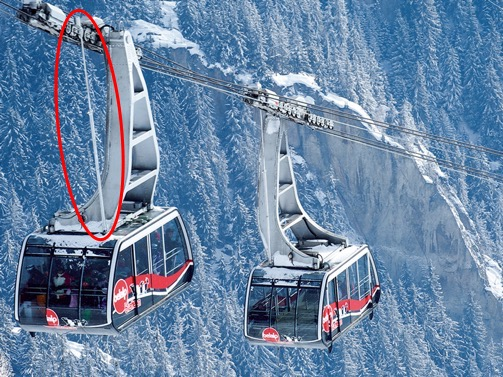
\includegraphics[width=\textwidth]{abbildung1.jpg}
    \caption{Dämpfung einer grossen Pendelbahnen per Gasfeder\protect\footnotemark}
    \label{fig:abb1}
\end{figure}
\footnotetext{\url{https://www.doppelmayr.com/uploads/tx\_vcs/Produkte-Pendelbahnen-Bildergalerie-ATWBlattenBelalp-Doppelmayr.jpg}}

\begin{figure}
    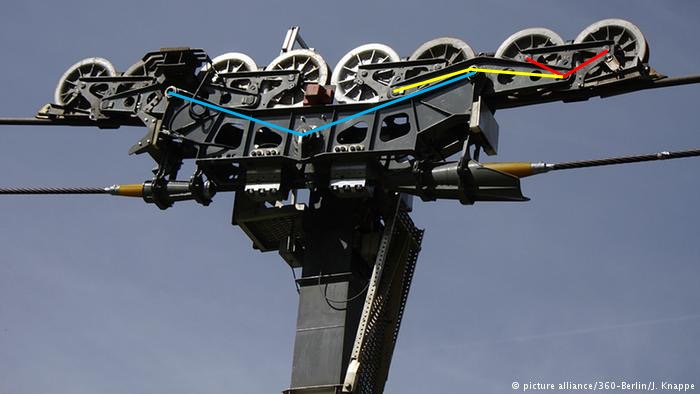
\includegraphics[width=\textwidth]{abbildung2.jpg}
    \caption{Über ein Brückensystem verbundene Laufrollen zur Anpassung der Rollen an die Krümmung des Tragseils}
    \label{fig:abb2}
\end{figure}

\begin{figure}
    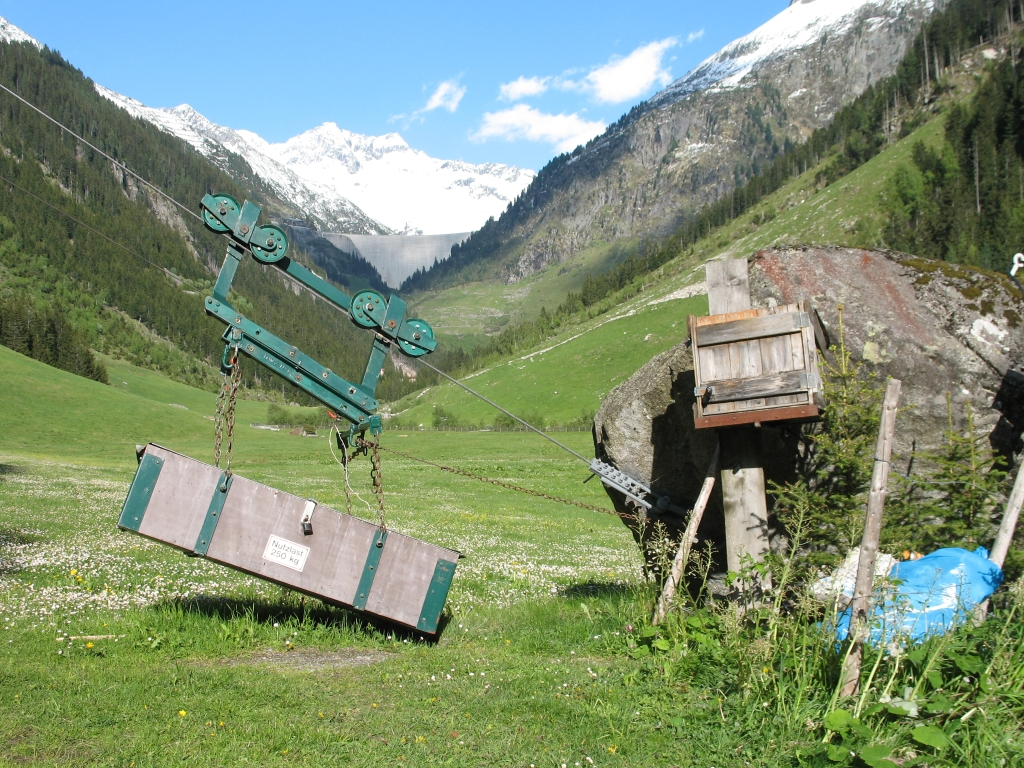
\includegraphics[width=\textwidth]{abbildung3.jpg}
    \caption{Schieflage der Arbeitsplattform aufgrund Aufhängung an zwei Punkten\protect\footnotemark}
    \label{fig:abb3}
\end{figure}
\footnotetext{\url{https://upload.wikimedia.org/wikipedia/commons/thumb/8/89/Materialseilbahn.jpg/800px-Materialseilbahn.jpg}}

\begin{figure}
    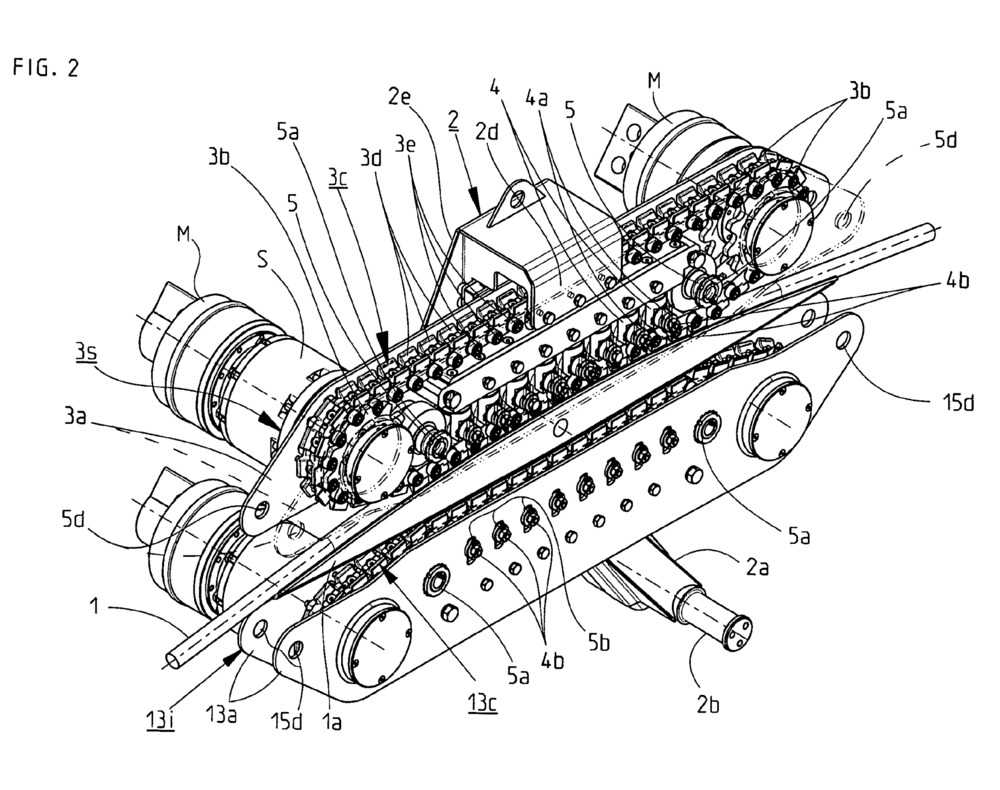
\includegraphics[width=\textwidth]{abbildung4.jpg}
    \caption{Patentierter Kettenantrieb direkt auf ein feststehendes Tragseil\protect\footnotemark}
    \label{fig:abb4}
\end{figure}
\footnotetext{\url{http://www.google.ch/patents/EP2527287A1?hl=de&cl=en}}

\subsection{Fazit}

\subsubsection{Bereich Maschinenbau}

Im Bereich Maschinenbau sind generell wenig für die Aufgabenstellung geeignete Informationen zu finden. Antriebe an einem einzelnen, stehenden Seil sind untypisch. Daher sind die Quellen beschränkt. Es sind jedoch hilfreiche Bilder und Videos vorhanden, die mögliche Lösungen zeigen. Auch von herkömmlichen Seilbahnen können Lösungsansätze abgeleitet werden. Quellen zu allgemeineren Themen, wie zum Beispiel Leichtbau, Seilreibung, Greifen von Objekten usw., sind in guter Qualität vorhanden.

\subsubsection{Bereich Elektrotechnik/Informatik}

Zu den Mikrocontrollern gibt es sehr viele Online-Ressourcen. Hier ist das Problem, dass man tendenziell eher zu viel als zu wenig findet. Auch bei den Software-Frameworks gibt es verschiedenste Varianten, was es schwierig macht, jedes einzelne zu evaluieren. Zu den beiden wohl am weitesten verbreiteten Mikrocontrollern Arduino und Raspberry Pi gibt es sehr viele Tutorials und Anleitungen darüber, wie man mit den Systemen umgeht, und wie man sie koppeln könnte. Jedoch sind nicht alle dieser Quellen wirklich hilfreich oder direkt auf unser Projekt anwendbar.

Bei den Sensoren gibt es viele gute Ressourcen zu verschiedenen Lösungen. Wir haben Anleitungen angeschaut, die beschreiben, wie mit dem Raspberry Pi Distanzen gemessen werden können. Für die Distanzmessung empfiehlt sich ein Ul\-tra\-schall-Sen\-sor. Dieser kostet lediglich ein paar Franken und ist bis auf ein paar Milimeter genau. Zusätzlich wurde angeschaut, wie die Bildverarbeitung mit dem Raspberry Pi funktioniert, und wie das erkannte Bild übertragen werden kann. Für die Bildverarbeitung scheint die OpenCV-Library geeignet zu sein, da diese selbst für komplizierte Aufgaben wie Gesichtserkennung eingesetzt werden kann. Die Erkennung eines Zielfeldes sollte also damit kein Problem darstellen.

Die technische Recherche zu den Motoren hat bisher zwei geeignete Motorenarten hervorgebracht, die es nun genauer zu betrachten gilt. Zum Thema Motorensteuerungen gibt es auch viele Quellen, hier sind jedoch nur Grundlagen aufgelistet, z.B. wie ein Servomotor und ein Schrittmotor funktioniert, und wie diese mit Arduino oder Raspberry Pi angesteuert werden können. Das gleiche gilt für die Stromversorgung. Hier wurden nur Grundlagen recherchiert und aufgelistet, die nicht ohne Weiteres auf unser Projekt anwendbar sind.

Zu der Lastaufnahme wurden diverse Möglichkeiten recherchiert: Greifarm, Elektromagnet oder ein Soft-Robotics-Greif\-arm. Es gibt eine Videoanleitung auf YouTube, die beschreibt, wie man einen solchen Soft-Robotics Greifarm selber aus Silikon baut. Generell müssen wir noch mehr recherchieren und noch mehr ins Detail gehen. Die Recherchen sind alle noch sehr grundlegend, da die Erfahrung mit solchen Systemen und Komponenten nicht vorhanden ist.  

\end{document}
